\documentclass[]{IEEEphot}
\jvol{1}
\jnum{1}
\jmonth{Marth}
\pubyear{2012}
\usepackage{graphicx}
\usepackage{amssymb}
\usepackage{fontspec}
\XeTeXlinebreaklocale "zh" %针对中文进行断行
\setmainfont{WenQuanYi Zen Hei} %设置默认的字体
\linespread{1.2}

\begin{document}
\title{数字图像处理实验二\\实验报告}
\author{040920112 戴一冕}
\maketitle
\markboth{数字图像处理}{实验二实验报告}
\begin{abstract}
  对给定实验图片进行直方图均衡化和直方图匹配等操作
\end{abstract}
\begin{IEEEkeywords}
	直方图均衡化,直方图匹配
\end{IEEEkeywords}
\section{实验目的}
通过上机实验的手段巩固课堂上所学的关于直方图均衡化和直方图匹配等图像增强技术的认识和了解,学会自行编写上述函数,感受不同的直方图增强技术对最终图像效果的影响。
\section{实验内容}
\subsection{方法技术介绍}
直方图处理能有有效的用于图像增强,而直方图更是多种空间域处理技术的基础。
灰度级为[0,L-1]范围的数字图像的直方图是离散函数$h(r_k)=n_k$,其中$r_k$是第$k$级灰度,$n_k$是图像中灰度级为$r_k$的像素个数。经常以图像中的总数(用$n$表示)来除它的每个值,以得到归一化的直方图。因此,一个归一化的直方图由$P(r_k)=\frac{n_k}{n}$给出,其中$k=0,1,\cdots,L-1$。简单地说,$P(r_k)$给出了灰度级为$r_k$发生的概率估计值,显然一个归一化的直方图的所有部分之和应该等于$1$。
\subsubsection{直方图均衡}
直方图均衡的思想就是使处理后的图像灰度分布均衡,这样图像的信息熵最大,图像也就得到了相应的增强。
故而,对于上文中的非均匀的密度函数$P_r(r)$经某个变换函数$s=T(r)$变换为均匀概率分布$P_s(s)$,$s$为变换后的图像灰度值。
由雅克比变换易得:
\begin{equation}
	P_s(s)ds=P_r(r)dr
	\label{eql}
\end{equation}
当直方图均衡化并归一化后,
\begin{equation}
	p_s(s)=1
	\label{eql}
\end{equation}
即:
\begin{equation}
	ds=P_r(r)dr
	\label{eql}
\end{equation}
其中$s$,$r$归一化的含义就是$r\in[0,1],s\in[0,1]$,对应matlab中的就是图像的double类型。
两边取积分:
\begin{equation}
	s=T_r=\int\limits_{0}^{r}P_r(\omega)d\omega
	\label{eql}
\end{equation}
变换后图像的灰度$s$就是原图像灰度级的概率密度函数的积分。
\subsubsection{直方图匹配}
直方图均衡能自动地确定变换函数,该函数寻求产生均匀直方图的输出图像。对于某些应用来说,采用均匀直方图的基本增强并不是最好的办法,尤其是有时可以指定希望处理的图像所具有的直方图形状,这种用于产生处理后特有直方图的图像的方法,称为直方图匹配,也叫直方图规定化。
\paragraph{方法推导}
$r,z$为连续灰度级(看成是连续随机变量$P_r(r),P_z(z)$为它们对应的连续概率密度。
$r$为输入图像的灰度级,$z$为输出图像的灰度级,输入图像的概率密度函数为$P_r(r)$,$P_z(z)$为希望输出图像具有的规定概率密度函数。
令$s$为一随机变量,且有
\begin{equation}
s=T(r)=\int\limits_{0}^{r}P_r(\omega)d\omega
\end{equation}
同时对希望输出的图像做直方图均衡化,有
\begin{equation}
s=G(z)=\int\limits_{0}^{z}P_z(t)dt
\end{equation}
$$\because s=G(z)$$
$$\therefore z=G^{-1}(s)$$
$$\because s=T(r)$$
\begin{equation}
\therefore z=G^{-1}(s)=G^{-1}[T(r)]
\end{equation}
故而直方图规定化的步骤为:
\begin{enumerate}
\item 由(5)式求$T(r)$
\item 由(6)式求$G(z)$
\item 求反变换$G^{-1}$
\item 对输入图像的所有像素应用(7)式得到输出图像
\end{enumerate}
\subsection{实验步骤}
\subsubsection{步骤1}
自己编写直方图均衡和直方图规定化函数,开始积累由自己编写的图像处理模块。
\subsubsection{步骤2}
将mountain.jpg图像读入,对其做直方图均衡化,作出处理前后的灰度直方图,将其保存在同一窗口。
\subsubsection{步骤3}
将mountain.jpg图像读入,按如下灰度变换函数对其做直方图匹配,作出处理前后的灰度直方图,将其保存在同一窗口。
\begin{equation}
n=
\left\{
\begin{array}{lr}
1400r,    & r\leq r\\
7000-310r & 5<r\leq 20\\
900-5r    & 20<r\leq 180\\
-1440+8r  & 180<r\leq 225\\
3060-12r  & 225<\leq 255
\end{array}
\right.
\end{equation}
\section{实验结果与分析}
\subsection{实验环境介绍}
本实验采用Python 2.7.2及其Numpy、Scipy、PIL、matplotlib,以及笔者自己编写的PyDIP模块,同时又用Matlab再实验了一次以用来对照。
\subsection{分析结果}
\subsubsection{步骤1}
按照定义写了直方图均衡化和直方图匹配的函数,分别命名为histeq和histmatch,并整合到了PyDIP模块。
\subsubsection{步骤2}
对原图进行直方图均衡化后,处理后的图像较原图对比度变强了,也更加清晰。并且将结果与Matlab下的对比,从下面两幅图中可以看出,在灰度值小于225左右的范围内,两种方法处理的直方图分布几乎相同,但在灰度值大于225的范围内,自己编写的histeq函数直方图分布密集,而Matlab较为稀疏。\\
\begin{figure}[h]
	\includegraphics[width=12pc]{mexp_2_2.eps}
	\caption{(a)步骤2 Matlab的histeq函数实验结果图}
\end{figure}
\begin{figure}[h]
	\centering
	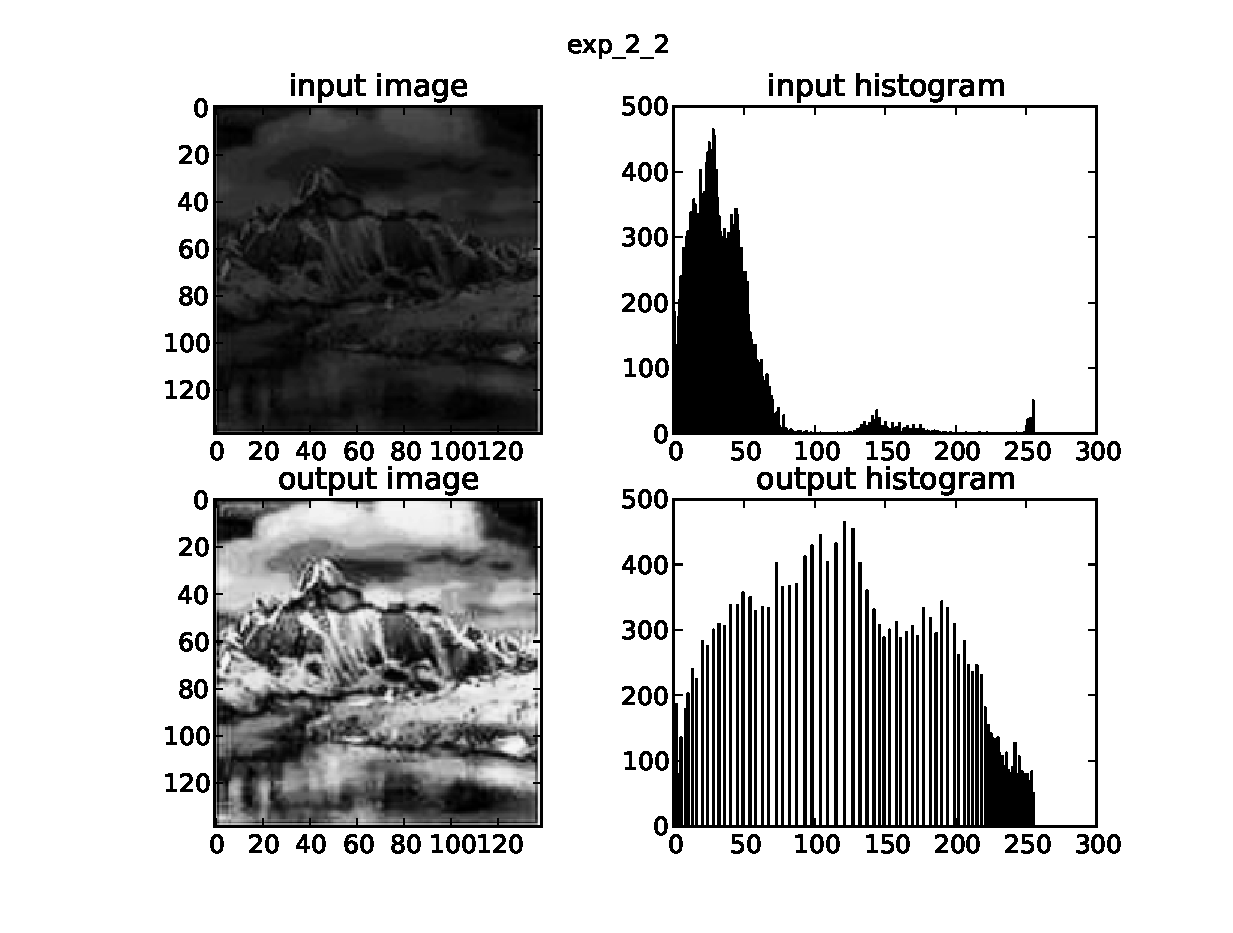
\includegraphics[width=30pc]{exp_2_2.eps}
	\caption{(b)步骤2 自己编写的histeq函数实验结果图}
\end{figure}
我按照课本上的定义计算了$s_k$的分布,发现$s_k$就是在灰度值大于225以后的这段范围内是密集分布的,因此可以证明我自己编写的histeq函数是没有错误的。那么Matlab的结果较为稀疏的原因应该是其采用了额外的优化算法。
\subsubsection{步骤3}
在该步骤中,我按照定义写了histmatch,并将实验结果与Matlab实现的相对照。对于处理后的图片,两者相差不大,肉眼很难分辨出,相比于原图像,对比度和清晰度都有了明显的改善。再比较两者的灰度直方图,虽然有稍许不同,但总的看来还是相近的。
\begin{figure}[h]
	\includegraphics[width=12pc]{mexp_2_3.eps}
	\caption{(c)步骤3 Matlab直方图匹配实验结果图}
\end{figure}
\begin{figure}[h]
	\centering
	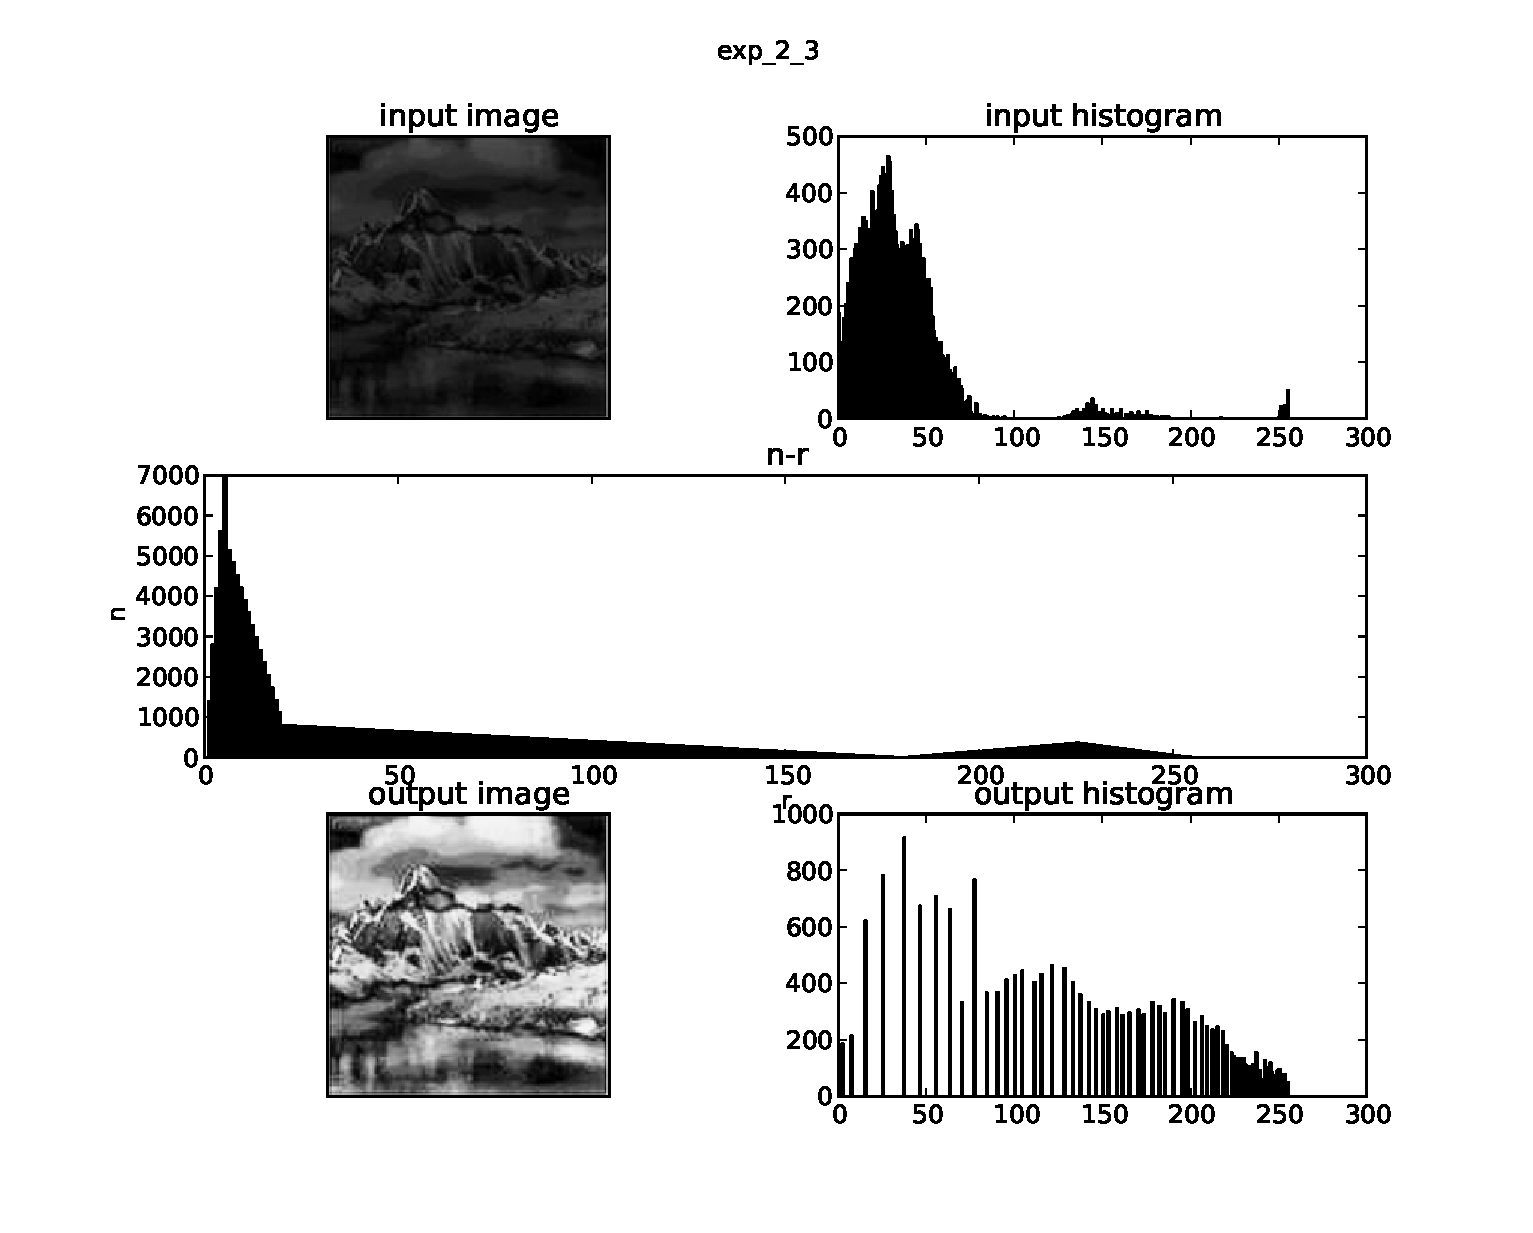
\includegraphics[width=30pc]{exp_2_3.eps}
	\caption{(d)步骤3 自己编写的histmatch实验结果图}
\end{figure}
\section{心得体会}
这次实验中需要编写直方图均衡和直方图匹配的函数,对于其实现过程,我分别花了两个晚自习来掌握,过程比较艰难,但在写出来之后,看到用自己写的histeq和histmatch的直方图,还是非常自豪的,更何况借此机会,我还巩固了课堂上讲过的知识,一举两得。
\section{实验程序}
实验程序附在随文的文件夹内。
\end{document}

